\documentclass[border=4pt]{standalone}
\usepackage{amsmath,amssymb,amsfonts}
\usepackage{xcolor,colortbl,array,booktabs,multirow}
\usepackage{tikz}
\usepackage{pgfplots}
\pgfplotsset{compat=1.16}
\usetikzlibrary{arrows, automata, backgrounds, calendar, chains, decorations,
    matrix, mindmap, patterns, petri, positioning, shadows, shapes.geometric,
    trees, shapes, decorations.pathreplacing, calc, tikzmark, arrows.meta,
    intersections, fit, graphs, quotes, angles, decorations.markings}
\newcommand{\st}{\text{ s.t. }}
\newcommand{\x}{\mathbf{x}}
\renewcommand{\b}{\mathbf{b}}
\renewcommand{\c}{\mathbf{c}}
\newcommand{\A}{\mathbf{A}}
\newcommand{\y}{\mathbf{y}}
\newcommand{\z}{\mathbf{z}}
\newcommand{\R}{\mathbb{R}}
\newcommand{\RR}{\mathbb{R}}
\newcommand{\Z}{\mathbb{Z}}
\newcommand{\ZZ}{\mathbb{Z}}
\newcommand{\npcomplete}{NP-complete}
\providecommand{\true}{\text{TRUE}}
\providecommand{\false}{\text{FALSE}}
\tikzset{vertex/.style={circle,fill=black!25,minimum size=20pt,inner sep=0pt},
    edge/.style={draw,thick,-},weight/.style={font=\small},
    selected vertex/.style={vertex, fill=red!24},
    selected edge/.style={draw,line width=2pt,-,red!50},
    ignored edge/.style={draw,line width=2pt,-,black!20}}
\newcommand{\vect}{\vec}
\providecommand{\ds}{\displaystyle}
\providecommand{\longvect}{\overrightarrow}
\usepackage[normalem]{ulem}
\definecolor{ocre}{RGB}{243,102,25}
\providecommand{\leftB}{\left[}
\providecommand{\rightB}{\right]}
\tikzset{directed/.style={postaction={decorate,decoration={markings,mark=at position .65 with {\arrow{>}}}}},
    directed1/.style={postaction={decorate,decoration={markings,mark=at position .65 with {\arrow{>}}}}}}
\begin{document}
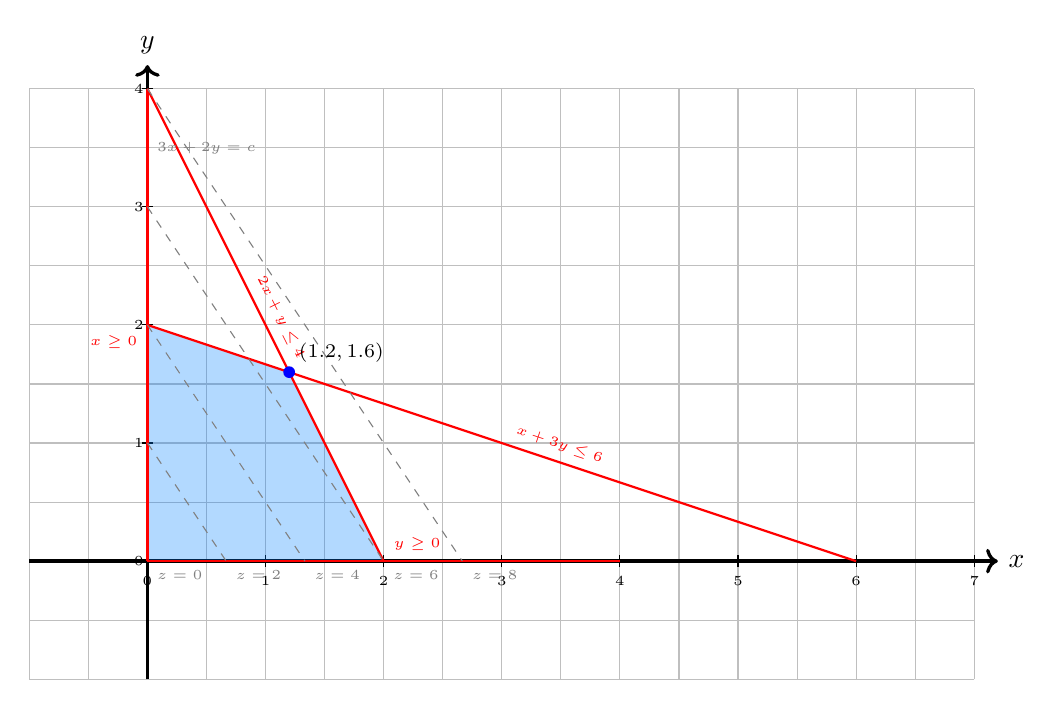
\begin{tikzpicture}[scale = 1.5]
    % Grid and axes
    \draw[gray!50, thin, step=0.5] (-1,-1) grid (7,4);
    \draw[very thick,->] (-1,0) -- (7.2,0) node[right] {$x$};
    \draw[very thick,->] (0,-1) -- (0,4.2) node[above] {$y$};

    % Axis labels
    \foreach \x in {0,...,7} \draw (\x,0.05) -- (\x,-0.05) node[below] {\tiny\x};
    \foreach \y in {0,...,4} \draw (-0.05,\y) -- (0.05,\y) node[left] {\tiny\y};

    % Shaded feasible region
    \fill[blue!50!cyan,opacity=0.3] (0,0) -- (0,2) -- (1.2,1.6) -- (2,0) -- cycle;

    % Constraint lines
    \draw[red,thick] (0,2) -- node[above right,sloped] {\tiny$x + 3y \leq 6$} (6,0);
    \draw[red,thick] (0,4) -- node[above,sloped] {\tiny$2x + y \leq 4$} (2,0);
    \draw[red,thick] (0,0) -- node[below left] {\tiny$x \geq 0$} (0,4);
    \draw[red,thick] (0,0) -- node[above right] {\tiny$y \geq 0$} (4,0);

        % Objective function contours
            \draw[dashed,gray] (0,4) -- (8/3,0) node[below right] {\tiny$z=8$};
    \draw[dashed,gray] (0,3) -- (2,0) node[below right] {\tiny$z=6$};
    \draw[dashed,gray] (0,2) -- (4/3,0) node[below right] {\tiny$z=4$};
    \draw[dashed,gray] (0,1) -- (2/3,0) node[below right] {\tiny$z=2$};
    \draw[dashed,gray] (0,0) -- (0,0) node[below right] {\tiny$z=0$};

    % Contour labels
    \node[gray] at (0.5,3.5) {\tiny$3x + 2y = c$};

     \node[blue] at (1.2,1.6) [circle,fill,inner sep=1.5pt]{};

    % Labels for vertices
    \node[black,anchor=south west] at (1.2,1.6) {\scriptsize$(1.2,1.6)$};
\end{tikzpicture}
\end{document}
